\documentclass[1p]{elsarticle_modified}
%\bibliographystyle{elsarticle-num}

%\usepackage[colorlinks]{hyperref}
%\usepackage{abbrmath_seonhwa} %\Abb, \Ascr, \Acal ,\Abf, \Afrak
\usepackage{amsfonts}
\usepackage{amssymb}
\usepackage{amsmath}
\usepackage{amsthm}
\usepackage{scalefnt}
\usepackage{amsbsy}
\usepackage{kotex}
\usepackage{caption}
\usepackage{subfig}
\usepackage{color}
\usepackage{graphicx}
\usepackage{xcolor} %% white, black, red, green, blue, cyan, magenta, yellow
\usepackage{float}
\usepackage{setspace}
\usepackage{hyperref}

\usepackage{tikz}
\usetikzlibrary{arrows}

\usepackage{multirow}
\usepackage{array} % fixed length table
\usepackage{hhline}

%%%%%%%%%%%%%%%%%%%%%
\makeatletter
\renewcommand*\env@matrix[1][\arraystretch]{%
	\edef\arraystretch{#1}%
	\hskip -\arraycolsep
	\let\@ifnextchar\new@ifnextchar
	\array{*\c@MaxMatrixCols c}}
\makeatother %https://tex.stackexchange.com/questions/14071/how-can-i-increase-the-line-spacing-in-a-matrix
%%%%%%%%%%%%%%%

\usepackage[normalem]{ulem}

\newcommand{\msout}[1]{\ifmmode\text{\sout{\ensuremath{#1}}}\else\sout{#1}\fi}
%SOURCE: \msout is \stkout macro in https://tex.stackexchange.com/questions/20609/strikeout-in-math-mode

\newcommand{\cancel}[1]{
	\ifmmode
	{\color{red}\msout{#1}}
	\else
	{\color{red}\sout{#1}}
	\fi
}

\newcommand{\add}[1]{
	{\color{blue}\uwave{#1}}
}

\newcommand{\replace}[2]{
	\ifmmode
	{\color{red}\msout{#1}}{\color{blue}\uwave{#2}}
	\else
	{\color{red}\sout{#1}}{\color{blue}\uwave{#2}}
	\fi
}

\newcommand{\Sol}{\mathcal{S}} %segment
\newcommand{\D}{D} %diagram
\newcommand{\A}{\mathcal{A}} %arc


%%%%%%%%%%%%%%%%%%%%%%%%%%%%%5 test

\def\sl{\operatorname{\textup{SL}}(2,\Cbb)}
\def\psl{\operatorname{\textup{PSL}}(2,\Cbb)}
\def\quan{\mkern 1mu \triangleright \mkern 1mu}

\theoremstyle{definition}
\newtheorem{thm}{Theorem}[section]
\newtheorem{prop}[thm]{Proposition}
\newtheorem{lem}[thm]{Lemma}
\newtheorem{ques}[thm]{Question}
\newtheorem{cor}[thm]{Corollary}
\newtheorem{defn}[thm]{Definition}
\newtheorem{exam}[thm]{Example}
\newtheorem{rmk}[thm]{Remark}
\newtheorem{alg}[thm]{Algorithm}

\newcommand{\I}{\sqrt{-1}}
\begin{document}

%\begin{frontmatter}
%
%\title{Boundary parabolic representations of knots up to 8 crossings}
%
%%% Group authors per affiliation:
%\author{Yunhi Cho} 
%\address{Department of Mathematics, University of Seoul, Seoul, Korea}
%\ead{yhcho@uos.ac.kr}
%
%
%\author{Seonhwa Kim} %\fnref{s_kim}}
%\address{Center for Geometry and Physics, Institute for Basic Science, Pohang, 37673, Korea}
%\ead{ryeona17@ibs.re.kr}
%
%\author{Hyuk Kim}
%\address{Department of Mathematical Sciences, Seoul National University, Seoul 08826, Korea}
%\ead{hyukkim@snu.ac.kr}
%
%\author{Seokbeom Yoon}
%\address{Department of Mathematical Sciences, Seoul National University, Seoul, 08826,  Korea}
%\ead{sbyoon15@snu.ac.kr}
%
%\begin{abstract}
%We find all boundary parabolic representation of knots up to 8 crossings.
%
%\end{abstract}
%\begin{keyword}
%    \MSC[2010] 57M25 
%\end{keyword}
%
%\end{frontmatter}

%\linenumbers
%\tableofcontents
%
\newcommand\colored[1]{\textcolor{white}{\rule[-0.35ex]{0.8em}{1.4ex}}\kern-0.8em\color{red} #1}%
%\newcommand\colored[1]{\textcolor{white}{ #1}\kern-2.17ex	\textcolor{white}{ #1}\kern-1.81ex	\textcolor{white}{ #1}\kern-2.15ex\color{red}#1	}

{\Large $\underline{12n_{0862}~(K12n_{0862})}$}

\setlength{\tabcolsep}{10pt}
\renewcommand{\arraystretch}{1.6}
\vspace{1cm}\begin{tabular}{m{100pt}>{\centering\arraybackslash}m{274pt}}
\multirow{5}{120pt}{
	\centering
	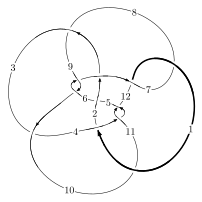
\includegraphics[width=112pt]{../../../GIT/diagram.site/Diagrams/png/2951_12n_0862.png}\\
\ \ \ A knot diagram\footnotemark}&
\allowdisplaybreaks
\textbf{Linearized knot diagam} \\
\cline{2-2}
 &
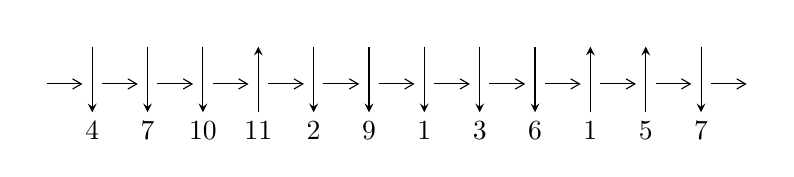
\begin{tikzpicture}[x=20pt, y=17pt]
	% nodes
	\node (C0) at (0, 0) {};
	\node (C1) at (1, 0) {};
	\node (C1U) at (1, +1) {};
	\node (C1D) at (1, -1) {4};

	\node (C2) at (2, 0) {};
	\node (C2U) at (2, +1) {};
	\node (C2D) at (2, -1) {7};

	\node (C3) at (3, 0) {};
	\node (C3U) at (3, +1) {};
	\node (C3D) at (3, -1) {10};

	\node (C4) at (4, 0) {};
	\node (C4U) at (4, +1) {};
	\node (C4D) at (4, -1) {11};

	\node (C5) at (5, 0) {};
	\node (C5U) at (5, +1) {};
	\node (C5D) at (5, -1) {2};

	\node (C6) at (6, 0) {};
	\node (C6U) at (6, +1) {};
	\node (C6D) at (6, -1) {9};

	\node (C7) at (7, 0) {};
	\node (C7U) at (7, +1) {};
	\node (C7D) at (7, -1) {1};

	\node (C8) at (8, 0) {};
	\node (C8U) at (8, +1) {};
	\node (C8D) at (8, -1) {3};

	\node (C9) at (9, 0) {};
	\node (C9U) at (9, +1) {};
	\node (C9D) at (9, -1) {6};

	\node (C10) at (10, 0) {};
	\node (C10U) at (10, +1) {};
	\node (C10D) at (10, -1) {1};

	\node (C11) at (11, 0) {};
	\node (C11U) at (11, +1) {};
	\node (C11D) at (11, -1) {5};

	\node (C12) at (12, 0) {};
	\node (C12U) at (12, +1) {};
	\node (C12D) at (12, -1) {7};
	\node (C13) at (13, 0) {};

	% arrows
	\draw[->,>={angle 60}]
	(C0) edge (C1) (C1) edge (C2) (C2) edge (C3) (C3) edge (C4) (C4) edge (C5) (C5) edge (C6) (C6) edge (C7) (C7) edge (C8) (C8) edge (C9) (C9) edge (C10) (C10) edge (C11) (C11) edge (C12) (C12) edge (C13) ;	\draw[->,>=stealth]
	(C1U) edge (C1D) (C2U) edge (C2D) (C3U) edge (C3D) (C4D) edge (C4U) (C5U) edge (C5D) (C6U) edge (C6D) (C7U) edge (C7D) (C8U) edge (C8D) (C9U) edge (C9D) (C10D) edge (C10U) (C11D) edge (C11U) (C12U) edge (C12D) ;
	\end{tikzpicture} \\
\hhline{~~} \\& 
\textbf{Solving Sequence} \\ \cline{2-2} 
 &
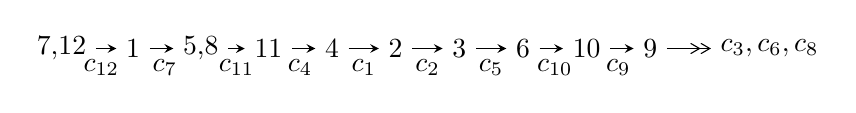
\begin{tikzpicture}[x=23pt, y=7pt]
	% node
	\node (A0) at (-1/8, 0) {7,12};
	\node (A1) at (1, 0) {1};
	\node (A2) at (33/16, 0) {5,8};
	\node (A3) at (25/8, 0) {11};
	\node (A4) at (33/8, 0) {4};
	\node (A5) at (41/8, 0) {2};
	\node (A6) at (49/8, 0) {3};
	\node (A7) at (57/8, 0) {6};
	\node (A8) at (65/8, 0) {10};
	\node (A9) at (73/8, 0) {9};
	\node (C1) at (1/2, -1) {$c_{12}$};
	\node (C2) at (3/2, -1) {$c_{7}$};
	\node (C3) at (21/8, -1) {$c_{11}$};
	\node (C4) at (29/8, -1) {$c_{4}$};
	\node (C5) at (37/8, -1) {$c_{1}$};
	\node (C6) at (45/8, -1) {$c_{2}$};
	\node (C7) at (53/8, -1) {$c_{5}$};
	\node (C8) at (61/8, -1) {$c_{10}$};
	\node (C9) at (69/8, -1) {$c_{9}$};
	\node (A10) at (11, 0) {$c_{3},c_{6},c_{8}$};

	% edge
	\draw[->,>=stealth]	
	(A0) edge (A1) (A1) edge (A2) (A2) edge (A3) (A3) edge (A4) (A4) edge (A5) (A5) edge (A6) (A6) edge (A7) (A7) edge (A8) (A8) edge (A9) ;
	\draw[->>,>={angle 60}]	
	(A9) edge (A10);
\end{tikzpicture} \\ 

\end{tabular} \\

\footnotetext{
The image of knot diagram is generated by the software ``\textbf{Draw programme}" developed by Andrew Bartholomew(\url{http://www.layer8.co.uk/maths/draw/index.htm\#Running-draw}), where we modified some parts for our purpose(\url{https://github.com/CATsTAILs/LinksPainter}).
}\phantom \\ \newline 
\centering \textbf{Ideals for irreducible components\footnotemark of $X_{\text{par}}$} 
 
\begin{align*}
I^u_{1}&=\langle 
-4.13423\times10^{545} u^{98}-8.41031\times10^{545} u^{97}+\cdots+7.71729\times10^{546} b-9.78140\times10^{546},\\
\phantom{I^u_{1}}&\phantom{= \langle  }5.62354\times10^{545} u^{98}+8.39082\times10^{545} u^{97}+\cdots+7.71729\times10^{546} a-1.14457\times10^{547},\;u^{99}+2 u^{98}+\cdots-14 u-1\rangle \\
I^u_{2}&=\langle 
1.44391\times10^{37} u^{35}-2.21652\times10^{37} u^{34}+\cdots+7.10926\times10^{36} b-1.15603\times10^{37},\\
\phantom{I^u_{2}}&\phantom{= \langle  }-2.43176\times10^{37} u^{35}+4.52865\times10^{37} u^{34}+\cdots+7.10926\times10^{36} a-4.98348\times10^{37},\;u^{36}- u^{35}+\cdots-2 u-1\rangle \\
\\
\end{align*}
\raggedright * 2 irreducible components of $\dim_{\mathbb{C}}=0$, with total 135 representations.\\
\footnotetext{All coefficients of polynomials are rational numbers. But the coefficients are sometimes approximated in decimal forms when there is not enough margin.}
\newpage
\renewcommand{\arraystretch}{1}
\centering \section*{I. $I^u_{1}= \langle -4.13\times10^{545} u^{98}-8.41\times10^{545} u^{97}+\cdots+7.72\times10^{546} b-9.78\times10^{546},\;5.62\times10^{545} u^{98}+8.39\times10^{545} u^{97}+\cdots+7.72\times10^{546} a-1.14\times10^{547},\;u^{99}+2 u^{98}+\cdots-14 u-1 \rangle$}
\flushleft \textbf{(i) Arc colorings}\\
\begin{tabular}{m{7pt} m{180pt} m{7pt} m{180pt} }
\flushright $a_{7}=$&$\begin{pmatrix}0\\u\end{pmatrix}$ \\
\flushright $a_{12}=$&$\begin{pmatrix}1\\0\end{pmatrix}$ \\
\flushright $a_{1}=$&$\begin{pmatrix}1\\u^2\end{pmatrix}$ \\
\flushright $a_{5}=$&$\begin{pmatrix}-0.0728693 u^{98}-0.108728 u^{97}+\cdots-13.0659 u+1.48313\\0.0535710 u^{98}+0.108980 u^{97}+\cdots-0.601675 u+1.26747\end{pmatrix}$ \\
\flushright $a_{8}=$&$\begin{pmatrix}- u\\- u^3+u\end{pmatrix}$ \\
\flushright $a_{11}=$&$\begin{pmatrix}0.0740548 u^{98}+0.178821 u^{97}+\cdots-11.5713 u+4.30161\\0.0862112 u^{98}+0.164238 u^{97}+\cdots+2.60025 u+1.58172\end{pmatrix}$ \\
\flushright $a_{4}=$&$\begin{pmatrix}-0.334497 u^{98}-0.626075 u^{97}+\cdots-12.9486 u-5.18044\\-0.0392665 u^{98}-0.0482840 u^{97}+\cdots-9.63437 u-0.506867\end{pmatrix}$ \\
\flushright $a_{2}=$&$\begin{pmatrix}-0.0956699 u^{98}-0.257464 u^{97}+\cdots+10.1109 u-5.80856\\0.00747297 u^{98}+0.0566310 u^{97}+\cdots-21.3422 u-3.34556\end{pmatrix}$ \\
\flushright $a_{3}=$&$\begin{pmatrix}-0.0956699 u^{98}-0.257464 u^{97}+\cdots+10.1109 u-5.80856\\0.0249836 u^{98}+0.0918021 u^{97}+\cdots-22.3636 u-3.41168\end{pmatrix}$ \\
\flushright $a_{6}=$&$\begin{pmatrix}0.787689 u^{98}+1.52752 u^{97}+\cdots-69.5405 u-9.45597\\0.0462208 u^{98}+0.110462 u^{97}+\cdots-15.8136 u-2.79226\end{pmatrix}$ \\
\flushright $a_{10}=$&$\begin{pmatrix}-0.0192983 u^{98}+0.000252513 u^{97}+\cdots-13.6676 u+2.75060\\0.0886812 u^{98}+0.169088 u^{97}+\cdots+2.62084 u+1.58986\end{pmatrix}$ \\
\flushright $a_{9}=$&$\begin{pmatrix}0.509611 u^{98}+0.950444 u^{97}+\cdots-68.2325 u+2.11639\\0.396273 u^{98}+0.765808 u^{97}+\cdots-26.1751 u-0.792660\end{pmatrix}$\\&\end{tabular}
\flushleft \textbf{(ii) Obstruction class $= -1$}\\~\\
\flushleft \textbf{(iii) Cusp Shapes $= -0.730846 u^{98}-1.26329 u^{97}+\cdots-88.2611 u-10.4029$}\\~\\
\newpage\renewcommand{\arraystretch}{1}
\flushleft \textbf{(iv) u-Polynomials at the component}\newline \\
\begin{tabular}{m{50pt}|m{274pt}}
Crossings & \hspace{64pt}u-Polynomials at each crossing \\
\hline $$\begin{aligned}c_{1}\end{aligned}$$&$\begin{aligned}
&u^{99}+8 u^{98}+\cdots+36 u-5
\end{aligned}$\\
\hline $$\begin{aligned}c_{2}\end{aligned}$$&$\begin{aligned}
&u^{99}- u^{98}+\cdots-20407938 u-31437685
\end{aligned}$\\
\hline $$\begin{aligned}c_{3}\end{aligned}$$&$\begin{aligned}
&u^{99}-2 u^{98}+\cdots-309043 u+44933
\end{aligned}$\\
\hline $$\begin{aligned}c_{4},c_{11}\end{aligned}$$&$\begin{aligned}
&u^{99}+2 u^{98}+\cdots+66361 u+6341
\end{aligned}$\\
\hline $$\begin{aligned}c_{5}\end{aligned}$$&$\begin{aligned}
&u^{99}-3 u^{98}+\cdots-439231 u-28927
\end{aligned}$\\
\hline $$\begin{aligned}c_{6},c_{9}\end{aligned}$$&$\begin{aligned}
&u^{99}-5 u^{98}+\cdots-544 u+88
\end{aligned}$\\
\hline $$\begin{aligned}c_{7},c_{12}\end{aligned}$$&$\begin{aligned}
&u^{99}+2 u^{98}+\cdots-14 u-1
\end{aligned}$\\
\hline $$\begin{aligned}c_{8}\end{aligned}$$&$\begin{aligned}
&u^{99}+u^{98}+\cdots+1415210 u-900451
\end{aligned}$\\
\hline $$\begin{aligned}c_{10}\end{aligned}$$&$\begin{aligned}
&u^{99}+6 u^{98}+\cdots-11704 u+191
\end{aligned}$\\
\hline
\end{tabular}\\~\\
\newpage\renewcommand{\arraystretch}{1}
\flushleft \textbf{(v) Riley Polynomials at the component}\newline \\
\begin{tabular}{m{50pt}|m{274pt}}
Crossings & \hspace{64pt}Riley Polynomials at each crossing \\
\hline $$\begin{aligned}c_{1}\end{aligned}$$&$\begin{aligned}
&y^{99}-10 y^{98}+\cdots-294 y-25
\end{aligned}$\\
\hline $$\begin{aligned}c_{2}\end{aligned}$$&$\begin{aligned}
&y^{99}+41 y^{98}+\cdots-24026013786433826 y-988328038159225
\end{aligned}$\\
\hline $$\begin{aligned}c_{3}\end{aligned}$$&$\begin{aligned}
&y^{99}+10 y^{98}+\cdots-1343708331 y-2018974489
\end{aligned}$\\
\hline $$\begin{aligned}c_{4},c_{11}\end{aligned}$$&$\begin{aligned}
&y^{99}-90 y^{98}+\cdots+1567376929 y-40208281
\end{aligned}$\\
\hline $$\begin{aligned}c_{5}\end{aligned}$$&$\begin{aligned}
&y^{99}+47 y^{98}+\cdots+82222035835 y-836771329
\end{aligned}$\\
\hline $$\begin{aligned}c_{6},c_{9}\end{aligned}$$&$\begin{aligned}
&y^{99}+59 y^{98}+\cdots-190880 y-7744
\end{aligned}$\\
\hline $$\begin{aligned}c_{7},c_{12}\end{aligned}$$&$\begin{aligned}
&y^{99}+88 y^{98}+\cdots-138 y-1
\end{aligned}$\\
\hline $$\begin{aligned}c_{8}\end{aligned}$$&$\begin{aligned}
&y^{99}+33 y^{98}+\cdots-28122811583158 y-810812003401
\end{aligned}$\\
\hline $$\begin{aligned}c_{10}\end{aligned}$$&$\begin{aligned}
&y^{99}-46 y^{98}+\cdots+118391676 y-36481
\end{aligned}$\\
\hline
\end{tabular}\\~\\
\newpage\flushleft \textbf{(vi) Complex Volumes and Cusp Shapes}
$$\begin{array}{c|c|c}  
\text{Solutions to }I^u_{1}& \I (\text{vol} + \sqrt{-1}CS) & \text{Cusp shape}\\
 \hline 
\begin{aligned}
u &= \phantom{-}0.841907 + 0.665859 I \\
a &= -0.480654 - 1.217040 I \\
b &= \phantom{-}1.174250 - 0.039744 I\end{aligned}
 & \phantom{-}2.49130 - 4.74543 I & \phantom{-0.000000 } 0 \\ \hline\begin{aligned}
u &= \phantom{-}0.841907 - 0.665859 I \\
a &= -0.480654 + 1.217040 I \\
b &= \phantom{-}1.174250 + 0.039744 I\end{aligned}
 & \phantom{-}2.49130 + 4.74543 I & \phantom{-0.000000 } 0 \\ \hline\begin{aligned}
u &= -0.558882 + 0.663005 I \\
a &= -0.546261 - 1.222320 I \\
b &= \phantom{-}0.502565 + 0.043849 I\end{aligned}
 & \phantom{-}0.13656 + 4.34462 I & \phantom{-0.000000 } 0 \\ \hline\begin{aligned}
u &= -0.558882 - 0.663005 I \\
a &= -0.546261 + 1.222320 I \\
b &= \phantom{-}0.502565 - 0.043849 I\end{aligned}
 & \phantom{-}0.13656 - 4.34462 I & \phantom{-0.000000 } 0 \\ \hline\begin{aligned}
u &= -0.131669 + 1.135030 I \\
a &= \phantom{-}0.223696 - 0.439525 I \\
b &= -0.458676 + 0.424837 I\end{aligned}
 & \phantom{-}2.27045 + 1.29976 I & \phantom{-0.000000 } 0 \\ \hline\begin{aligned}
u &= -0.131669 - 1.135030 I \\
a &= \phantom{-}0.223696 + 0.439525 I \\
b &= -0.458676 - 0.424837 I\end{aligned}
 & \phantom{-}2.27045 - 1.29976 I & \phantom{-0.000000 } 0 \\ \hline\begin{aligned}
u &= -1.138660 + 0.274741 I \\
a &= \phantom{-}0.737094 - 0.887941 I \\
b &= \phantom{-}0.330996 - 0.935799 I\end{aligned}
 & -2.60891 + 0.42160 I & \phantom{-0.000000 } 0 \\ \hline\begin{aligned}
u &= -1.138660 - 0.274741 I \\
a &= \phantom{-}0.737094 + 0.887941 I \\
b &= \phantom{-}0.330996 + 0.935799 I\end{aligned}
 & -2.60891 - 0.42160 I & \phantom{-0.000000 } 0 \\ \hline\begin{aligned}
u &= \phantom{-}0.025254 + 1.180590 I \\
a &= \phantom{-}0.307410 + 0.482375 I \\
b &= -0.329710 - 0.747157 I\end{aligned}
 & \phantom{-}3.11063 - 2.43594 I & \phantom{-0.000000 } 0 \\ \hline\begin{aligned}
u &= \phantom{-}0.025254 - 1.180590 I \\
a &= \phantom{-}0.307410 - 0.482375 I \\
b &= -0.329710 + 0.747157 I\end{aligned}
 & \phantom{-}3.11063 + 2.43594 I & \phantom{-0.000000 } 0\\
 \hline 
 \end{array}$$\newpage$$\begin{array}{c|c|c}  
\text{Solutions to }I^u_{1}& \I (\text{vol} + \sqrt{-1}CS) & \text{Cusp shape}\\
 \hline 
\begin{aligned}
u &= \phantom{-}0.806800 + 0.101225 I \\
a &= \phantom{-}2.51629 - 0.95511 I \\
b &= \phantom{-}0.383951 - 0.268064 I\end{aligned}
 & -0.33641 - 6.65531 I & \phantom{-0.000000 } 0 \\ \hline\begin{aligned}
u &= \phantom{-}0.806800 - 0.101225 I \\
a &= \phantom{-}2.51629 + 0.95511 I \\
b &= \phantom{-}0.383951 + 0.268064 I\end{aligned}
 & -0.33641 + 6.65531 I & \phantom{-0.000000 } 0 \\ \hline\begin{aligned}
u &= \phantom{-}1.130000 + 0.503781 I \\
a &= -0.02556 - 1.90378 I \\
b &= \phantom{-}0.912448 - 0.703140 I\end{aligned}
 & -0.94367 - 6.59640 I & \phantom{-0.000000 } 0 \\ \hline\begin{aligned}
u &= \phantom{-}1.130000 - 0.503781 I \\
a &= -0.02556 + 1.90378 I \\
b &= \phantom{-}0.912448 + 0.703140 I\end{aligned}
 & -0.94367 + 6.59640 I & \phantom{-0.000000 } 0 \\ \hline\begin{aligned}
u &= -0.749780\phantom{ +0.000000I} \\
a &= \phantom{-}3.85347\phantom{ +0.000000I} \\
b &= \phantom{-}0.507829\phantom{ +0.000000I}\end{aligned}
 & -4.28603\phantom{ +0.000000I} & \phantom{-0.000000 } 0 \\ \hline\begin{aligned}
u &= -0.172092 + 1.243830 I \\
a &= -0.174890 - 0.489493 I \\
b &= -0.361805 - 0.145036 I\end{aligned}
 & \phantom{-}2.59575 + 2.23609 I & \phantom{-0.000000 } 0 \\ \hline\begin{aligned}
u &= -0.172092 - 1.243830 I \\
a &= -0.174890 + 0.489493 I \\
b &= -0.361805 + 0.145036 I\end{aligned}
 & \phantom{-}2.59575 - 2.23609 I & \phantom{-0.000000 } 0 \\ \hline\begin{aligned}
u &= \phantom{-}0.734114\phantom{ +0.000000I} \\
a &= -2.17128\phantom{ +0.000000I} \\
b &= \phantom{-}0.731388\phantom{ +0.000000I}\end{aligned}
 & -2.34784\phantom{ +0.000000I} & \phantom{-0.000000 } 0 \\ \hline\begin{aligned}
u &= -0.678779 + 0.269082 I \\
a &= \phantom{-}1.23135 + 0.81607 I \\
b &= \phantom{-}1.272410 - 0.203025 I\end{aligned}
 & -0.912418 - 0.160739 I & \phantom{-0.000000 } 0 \\ \hline\begin{aligned}
u &= -0.678779 - 0.269082 I \\
a &= \phantom{-}1.23135 - 0.81607 I \\
b &= \phantom{-}1.272410 + 0.203025 I\end{aligned}
 & -0.912418 + 0.160739 I & \phantom{-0.000000 } 0\\
 \hline 
 \end{array}$$\newpage$$\begin{array}{c|c|c}  
\text{Solutions to }I^u_{1}& \I (\text{vol} + \sqrt{-1}CS) & \text{Cusp shape}\\
 \hline 
\begin{aligned}
u &= \phantom{-}1.275020 + 0.163285 I \\
a &= -0.897049 + 0.290257 I \\
b &= \phantom{-}0.813600 + 0.085835 I\end{aligned}
 & -3.31462 - 1.01409 I & \phantom{-0.000000 } 0 \\ \hline\begin{aligned}
u &= \phantom{-}1.275020 - 0.163285 I \\
a &= -0.897049 - 0.290257 I \\
b &= \phantom{-}0.813600 - 0.085835 I\end{aligned}
 & -3.31462 + 1.01409 I & \phantom{-0.000000 } 0 \\ \hline\begin{aligned}
u &= \phantom{-}0.366152 + 0.612502 I \\
a &= \phantom{-}0.495378 + 0.200281 I \\
b &= -0.961051 + 0.092169 I\end{aligned}
 & \phantom{-}3.17315 + 0.57771 I & \phantom{-0.000000 } 0 \\ \hline\begin{aligned}
u &= \phantom{-}0.366152 - 0.612502 I \\
a &= \phantom{-}0.495378 - 0.200281 I \\
b &= -0.961051 - 0.092169 I\end{aligned}
 & \phantom{-}3.17315 - 0.57771 I & \phantom{-0.000000 } 0 \\ \hline\begin{aligned}
u &= \phantom{-}0.320047 + 0.620159 I \\
a &= \phantom{-}0.497009 - 0.267226 I \\
b &= -0.981853 - 0.461824 I\end{aligned}
 & \phantom{-}1.49843 + 1.71620 I & \phantom{-0.000000 } 0 \\ \hline\begin{aligned}
u &= \phantom{-}0.320047 - 0.620159 I \\
a &= \phantom{-}0.497009 + 0.267226 I \\
b &= -0.981853 + 0.461824 I\end{aligned}
 & \phantom{-}1.49843 - 1.71620 I & \phantom{-0.000000 } 0 \\ \hline\begin{aligned}
u &= -1.364920 + 0.022663 I \\
a &= -0.660886 + 0.261525 I \\
b &= \phantom{-}0.914002 + 0.084661 I\end{aligned}
 & -2.92110 + 1.72300 I & \phantom{-0.000000 } 0 \\ \hline\begin{aligned}
u &= -1.364920 - 0.022663 I \\
a &= -0.660886 - 0.261525 I \\
b &= \phantom{-}0.914002 - 0.084661 I\end{aligned}
 & -2.92110 - 1.72300 I & \phantom{-0.000000 } 0 \\ \hline\begin{aligned}
u &= -0.077138 + 1.372770 I \\
a &= \phantom{-}0.091199 - 0.752761 I \\
b &= -0.705516 - 0.513272 I\end{aligned}
 & \phantom{-}2.36200 + 2.20848 I & \phantom{-0.000000 } 0 \\ \hline\begin{aligned}
u &= -0.077138 - 1.372770 I \\
a &= \phantom{-}0.091199 + 0.752761 I \\
b &= -0.705516 + 0.513272 I\end{aligned}
 & \phantom{-}2.36200 - 2.20848 I & \phantom{-0.000000 } 0\\
 \hline 
 \end{array}$$\newpage$$\begin{array}{c|c|c}  
\text{Solutions to }I^u_{1}& \I (\text{vol} + \sqrt{-1}CS) & \text{Cusp shape}\\
 \hline 
\begin{aligned}
u &= \phantom{-}0.115603 + 1.381960 I \\
a &= \phantom{-}0.71542 + 1.29686 I \\
b &= -1.037720 + 0.412533 I\end{aligned}
 & \phantom{-}7.34093 - 7.61660 I & \phantom{-0.000000 } 0 \\ \hline\begin{aligned}
u &= \phantom{-}0.115603 - 1.381960 I \\
a &= \phantom{-}0.71542 - 1.29686 I \\
b &= -1.037720 - 0.412533 I\end{aligned}
 & \phantom{-}7.34093 + 7.61660 I & \phantom{-0.000000 } 0 \\ \hline\begin{aligned}
u &= -1.390590 + 0.253299 I \\
a &= \phantom{-}0.504938 - 0.165887 I \\
b &= -1.340510 - 0.191286 I\end{aligned}
 & \phantom{-}7.70793 - 0.30774 I & \phantom{-0.000000 } 0 \\ \hline\begin{aligned}
u &= -1.390590 - 0.253299 I \\
a &= \phantom{-}0.504938 + 0.165887 I \\
b &= -1.340510 + 0.191286 I\end{aligned}
 & \phantom{-}7.70793 + 0.30774 I & \phantom{-0.000000 } 0 \\ \hline\begin{aligned}
u &= \phantom{-}0.34035 + 1.37755 I \\
a &= -0.206775 + 0.498668 I \\
b &= -0.096627 + 0.445266 I\end{aligned}
 & \phantom{-}6.77160 - 6.21356 I & \phantom{-0.000000 } 0 \\ \hline\begin{aligned}
u &= \phantom{-}0.34035 - 1.37755 I \\
a &= -0.206775 - 0.498668 I \\
b &= -0.096627 - 0.445266 I\end{aligned}
 & \phantom{-}6.77160 + 6.21356 I & \phantom{-0.000000 } 0 \\ \hline\begin{aligned}
u &= -0.526678\phantom{ +0.000000I} \\
a &= \phantom{-}0.943179\phantom{ +0.000000I} \\
b &= \phantom{-}0.689513\phantom{ +0.000000I}\end{aligned}
 & -0.952013\phantom{ +0.000000I} & -10.9550\phantom{ +0.000000I} \\ \hline\begin{aligned}
u &= \phantom{-}0.35927 + 1.43517 I \\
a &= \phantom{-}0.373171 - 0.175529 I \\
b &= -0.178657 + 1.370660 I\end{aligned}
 & \phantom{-}7.48264 - 0.43702 I & \phantom{-0.000000 } 0 \\ \hline\begin{aligned}
u &= \phantom{-}0.35927 - 1.43517 I \\
a &= \phantom{-}0.373171 + 0.175529 I \\
b &= -0.178657 - 1.370660 I\end{aligned}
 & \phantom{-}7.48264 + 0.43702 I & \phantom{-0.000000 } 0 \\ \hline\begin{aligned}
u &= \phantom{-}0.487130 + 0.161889 I \\
a &= \phantom{-}2.74918 - 1.16574 I \\
b &= \phantom{-}1.359750 - 0.032280 I\end{aligned}
 & \phantom{-}3.15153 + 5.69737 I & \phantom{-}0.323090 - 1.093045 I\\
 \hline 
 \end{array}$$\newpage$$\begin{array}{c|c|c}  
\text{Solutions to }I^u_{1}& \I (\text{vol} + \sqrt{-1}CS) & \text{Cusp shape}\\
 \hline 
\begin{aligned}
u &= \phantom{-}0.487130 - 0.161889 I \\
a &= \phantom{-}2.74918 + 1.16574 I \\
b &= \phantom{-}1.359750 + 0.032280 I\end{aligned}
 & \phantom{-}3.15153 - 5.69737 I & \phantom{-}0.323090 + 1.093045 I \\ \hline\begin{aligned}
u &= \phantom{-}0.503721 + 0.078772 I \\
a &= \phantom{-}1.59142 - 0.27337 I \\
b &= \phantom{-}0.217966 - 0.535658 I\end{aligned}
 & \phantom{-}2.94519 + 2.79350 I & -5.37825 - 2.60185 I \\ \hline\begin{aligned}
u &= \phantom{-}0.503721 - 0.078772 I \\
a &= \phantom{-}1.59142 + 0.27337 I \\
b &= \phantom{-}0.217966 + 0.535658 I\end{aligned}
 & \phantom{-}2.94519 - 2.79350 I & -5.37825 + 2.60185 I \\ \hline\begin{aligned}
u &= -0.283860 + 0.380766 I \\
a &= \phantom{-}1.212560 + 0.571324 I \\
b &= \phantom{-}0.640597 - 0.599069 I\end{aligned}
 & -1.100560 - 0.006892 I & -10.45174 + 0.21085 I \\ \hline\begin{aligned}
u &= -0.283860 - 0.380766 I \\
a &= \phantom{-}1.212560 - 0.571324 I \\
b &= \phantom{-}0.640597 + 0.599069 I\end{aligned}
 & -1.100560 + 0.006892 I & -10.45174 - 0.21085 I \\ \hline\begin{aligned}
u &= \phantom{-}0.14706 + 1.52666 I \\
a &= -0.012539 + 0.419450 I \\
b &= -0.413730 + 0.752092 I\end{aligned}
 & \phantom{-}5.56058 + 3.23730 I & \phantom{-0.000000 } 0 \\ \hline\begin{aligned}
u &= \phantom{-}0.14706 - 1.52666 I \\
a &= -0.012539 - 0.419450 I \\
b &= -0.413730 - 0.752092 I\end{aligned}
 & \phantom{-}5.56058 - 3.23730 I & \phantom{-0.000000 } 0 \\ \hline\begin{aligned}
u &= \phantom{-}0.12041 + 1.55906 I \\
a &= \phantom{-}1.71311 + 0.59107 I \\
b &= -1.364850 + 0.053351 I\end{aligned}
 & \phantom{-}11.04790 + 4.75147 I & \phantom{-0.000000 } 0 \\ \hline\begin{aligned}
u &= \phantom{-}0.12041 - 1.55906 I \\
a &= \phantom{-}1.71311 - 0.59107 I \\
b &= -1.364850 - 0.053351 I\end{aligned}
 & \phantom{-}11.04790 - 4.75147 I & \phantom{-0.000000 } 0 \\ \hline\begin{aligned}
u &= \phantom{-}1.59446 + 0.11781 I \\
a &= \phantom{-}0.470296 - 0.148956 I \\
b &= -1.42228 - 0.28677 I\end{aligned}
 & \phantom{-}3.02276 + 3.67171 I & \phantom{-0.000000 } 0\\
 \hline 
 \end{array}$$\newpage$$\begin{array}{c|c|c}  
\text{Solutions to }I^u_{1}& \I (\text{vol} + \sqrt{-1}CS) & \text{Cusp shape}\\
 \hline 
\begin{aligned}
u &= \phantom{-}1.59446 - 0.11781 I \\
a &= \phantom{-}0.470296 + 0.148956 I \\
b &= -1.42228 + 0.28677 I\end{aligned}
 & \phantom{-}3.02276 - 3.67171 I & \phantom{-0.000000 } 0 \\ \hline\begin{aligned}
u &= \phantom{-}0.04772 + 1.60438 I \\
a &= \phantom{-}1.367460 + 0.152126 I \\
b &= -1.54935 + 0.63664 I\end{aligned}
 & \phantom{-}12.06290 - 7.00092 I & \phantom{-0.000000 } 0 \\ \hline\begin{aligned}
u &= \phantom{-}0.04772 - 1.60438 I \\
a &= \phantom{-}1.367460 - 0.152126 I \\
b &= -1.54935 - 0.63664 I\end{aligned}
 & \phantom{-}12.06290 + 7.00092 I & \phantom{-0.000000 } 0 \\ \hline\begin{aligned}
u &= -0.01871 + 1.60873 I \\
a &= -1.61348 + 0.03894 I \\
b &= \phantom{-}1.58139 - 0.02708 I\end{aligned}
 & \phantom{-}10.52470 - 0.08002 I & \phantom{-0.000000 } 0 \\ \hline\begin{aligned}
u &= -0.01871 - 1.60873 I \\
a &= -1.61348 - 0.03894 I \\
b &= \phantom{-}1.58139 + 0.02708 I\end{aligned}
 & \phantom{-}10.52470 + 0.08002 I & \phantom{-0.000000 } 0 \\ \hline\begin{aligned}
u &= -0.04319 + 1.61215 I \\
a &= \phantom{-}1.90412 - 0.14400 I \\
b &= -1.240570 + 0.030624 I\end{aligned}
 & \phantom{-}5.52663 - 2.36605 I & \phantom{-0.000000 } 0 \\ \hline\begin{aligned}
u &= -0.04319 - 1.61215 I \\
a &= \phantom{-}1.90412 + 0.14400 I \\
b &= -1.240570 - 0.030624 I\end{aligned}
 & \phantom{-}5.52663 + 2.36605 I & \phantom{-0.000000 } 0 \\ \hline\begin{aligned}
u &= \phantom{-}0.09411 + 1.62140 I \\
a &= \phantom{-}1.57411 + 0.01957 I \\
b &= -1.311230 - 0.324208 I\end{aligned}
 & \phantom{-}6.50816 + 6.43237 I & \phantom{-0.000000 } 0 \\ \hline\begin{aligned}
u &= \phantom{-}0.09411 - 1.62140 I \\
a &= \phantom{-}1.57411 - 0.01957 I \\
b &= -1.311230 + 0.324208 I\end{aligned}
 & \phantom{-}6.50816 - 6.43237 I & \phantom{-0.000000 } 0 \\ \hline\begin{aligned}
u &= -0.40126 + 1.58028 I \\
a &= \phantom{-}0.315133 + 0.055054 I \\
b &= -0.25564 - 1.43131 I\end{aligned}
 & \phantom{-}2.35561 + 5.41845 I & \phantom{-0.000000 } 0\\
 \hline 
 \end{array}$$\newpage$$\begin{array}{c|c|c}  
\text{Solutions to }I^u_{1}& \I (\text{vol} + \sqrt{-1}CS) & \text{Cusp shape}\\
 \hline 
\begin{aligned}
u &= -0.40126 - 1.58028 I \\
a &= \phantom{-}0.315133 - 0.055054 I \\
b &= -0.25564 + 1.43131 I\end{aligned}
 & \phantom{-}2.35561 - 5.41845 I & \phantom{-0.000000 } 0 \\ \hline\begin{aligned}
u &= -0.09574 + 1.63425 I \\
a &= \phantom{-}1.65669 - 0.13609 I \\
b &= -1.297230 + 0.168492 I\end{aligned}
 & \phantom{-}5.38317 - 3.33321 I & \phantom{-0.000000 } 0 \\ \hline\begin{aligned}
u &= -0.09574 - 1.63425 I \\
a &= \phantom{-}1.65669 + 0.13609 I \\
b &= -1.297230 - 0.168492 I\end{aligned}
 & \phantom{-}5.38317 + 3.33321 I & \phantom{-0.000000 } 0 \\ \hline\begin{aligned}
u &= \phantom{-}0.32785 + 1.60601 I \\
a &= \phantom{-}0.245188 - 0.074585 I \\
b &= -0.27399 + 1.39829 I\end{aligned}
 & \phantom{-}5.94803 - 11.21930 I & \phantom{-0.000000 } 0 \\ \hline\begin{aligned}
u &= \phantom{-}0.32785 - 1.60601 I \\
a &= \phantom{-}0.245188 + 0.074585 I \\
b &= -0.27399 - 1.39829 I\end{aligned}
 & \phantom{-}5.94803 + 11.21930 I & \phantom{-0.000000 } 0 \\ \hline\begin{aligned}
u &= -0.15468 + 1.66146 I \\
a &= \phantom{-}1.374040 - 0.309901 I \\
b &= -1.52586 + 0.10620 I\end{aligned}
 & \phantom{-}7.11961 - 5.54819 I & \phantom{-0.000000 } 0 \\ \hline\begin{aligned}
u &= -0.15468 - 1.66146 I \\
a &= \phantom{-}1.374040 + 0.309901 I \\
b &= -1.52586 - 0.10620 I\end{aligned}
 & \phantom{-}7.11961 + 5.54819 I & \phantom{-0.000000 } 0 \\ \hline\begin{aligned}
u &= -0.71253 + 1.55073 I \\
a &= -1.36949 + 0.72327 I \\
b &= \phantom{-}1.48889 + 0.52726 I\end{aligned}
 & \phantom{-}12.8693 + 6.8764 I & \phantom{-0.000000 } 0 \\ \hline\begin{aligned}
u &= -0.71253 - 1.55073 I \\
a &= -1.36949 - 0.72327 I \\
b &= \phantom{-}1.48889 - 0.52726 I\end{aligned}
 & \phantom{-}12.8693 - 6.8764 I & \phantom{-0.000000 } 0 \\ \hline\begin{aligned}
u &= -0.04063 + 1.70758 I \\
a &= \phantom{-}1.278400 - 0.060583 I \\
b &= -1.75827 - 0.48827 I\end{aligned}
 & \phantom{-}7.56157 + 3.30858 I & \phantom{-0.000000 } 0\\
 \hline 
 \end{array}$$\newpage$$\begin{array}{c|c|c}  
\text{Solutions to }I^u_{1}& \I (\text{vol} + \sqrt{-1}CS) & \text{Cusp shape}\\
 \hline 
\begin{aligned}
u &= -0.04063 - 1.70758 I \\
a &= \phantom{-}1.278400 + 0.060583 I \\
b &= -1.75827 + 0.48827 I\end{aligned}
 & \phantom{-}7.56157 - 3.30858 I & \phantom{-0.000000 } 0 \\ \hline\begin{aligned}
u &= \phantom{-}0.09804 + 1.70887 I \\
a &= \phantom{-}1.322810 + 0.138996 I \\
b &= -1.58383 - 0.20996 I\end{aligned}
 & \phantom{-}6.40985 + 3.35174 I & \phantom{-0.000000 } 0 \\ \hline\begin{aligned}
u &= \phantom{-}0.09804 - 1.70887 I \\
a &= \phantom{-}1.322810 - 0.138996 I \\
b &= -1.58383 + 0.20996 I\end{aligned}
 & \phantom{-}6.40985 - 3.35174 I & \phantom{-0.000000 } 0 \\ \hline\begin{aligned}
u &= -0.078333 + 0.268938 I \\
a &= \phantom{-}2.24092 - 1.99047 I \\
b &= \phantom{-}0.835453 + 0.478092 I\end{aligned}
 & -0.24867 + 4.16049 I & -7.66355 - 7.49884 I \\ \hline\begin{aligned}
u &= -0.078333 - 0.268938 I \\
a &= \phantom{-}2.24092 + 1.99047 I \\
b &= \phantom{-}0.835453 - 0.478092 I\end{aligned}
 & -0.24867 - 4.16049 I & -7.66355 + 7.49884 I \\ \hline\begin{aligned}
u &= \phantom{-}0.21066 + 1.72405 I \\
a &= \phantom{-}1.165180 + 0.153518 I \\
b &= -1.94902 + 0.92546 I\end{aligned}
 & \phantom{-}9.84065 + 2.24703 I & \phantom{-0.000000 } 0 \\ \hline\begin{aligned}
u &= \phantom{-}0.21066 - 1.72405 I \\
a &= \phantom{-}1.165180 - 0.153518 I \\
b &= -1.94902 - 0.92546 I\end{aligned}
 & \phantom{-}9.84065 - 2.24703 I & \phantom{-0.000000 } 0 \\ \hline\begin{aligned}
u &= \phantom{-}0.206008 + 0.095507 I \\
a &= \phantom{-}4.40218 + 1.16103 I \\
b &= \phantom{-}1.149320 - 0.378794 I\end{aligned}
 & \phantom{-}5.56039 - 6.41977 I & -1.64714 + 6.90816 I \\ \hline\begin{aligned}
u &= \phantom{-}0.206008 - 0.095507 I \\
a &= \phantom{-}4.40218 - 1.16103 I \\
b &= \phantom{-}1.149320 + 0.378794 I\end{aligned}
 & \phantom{-}5.56039 + 6.41977 I & -1.64714 - 6.90816 I \\ \hline\begin{aligned}
u &= \phantom{-}0.76917 + 1.60242 I \\
a &= -1.173590 - 0.564908 I \\
b &= \phantom{-}1.392800 - 0.185453 I\end{aligned}
 & \phantom{-}8.15426 - 4.21056 I & \phantom{-0.000000 } 0\\
 \hline 
 \end{array}$$\newpage$$\begin{array}{c|c|c}  
\text{Solutions to }I^u_{1}& \I (\text{vol} + \sqrt{-1}CS) & \text{Cusp shape}\\
 \hline 
\begin{aligned}
u &= \phantom{-}0.76917 - 1.60242 I \\
a &= -1.173590 + 0.564908 I \\
b &= \phantom{-}1.392800 + 0.185453 I\end{aligned}
 & \phantom{-}8.15426 + 4.21056 I & \phantom{-0.000000 } 0 \\ \hline\begin{aligned}
u &= -0.110856 + 0.169303 I \\
a &= \phantom{-}1.76909 - 0.13498 I \\
b &= \phantom{-}0.382443 + 0.713139 I\end{aligned}
 & -1.02164 - 2.30830 I & -7.48322 - 1.56595 I \\ \hline\begin{aligned}
u &= -0.110856 - 0.169303 I \\
a &= \phantom{-}1.76909 + 0.13498 I \\
b &= \phantom{-}0.382443 - 0.713139 I\end{aligned}
 & -1.02164 + 2.30830 I & -7.48322 + 1.56595 I \\ \hline\begin{aligned}
u &= -0.063091 + 0.187939 I \\
a &= \phantom{-}1.72582 + 0.32469 I \\
b &= \phantom{-}0.494125 - 0.690437 I\end{aligned}
 & -1.67668 - 0.04041 I & -5.30445 + 0.32910 I \\ \hline\begin{aligned}
u &= -0.063091 - 0.187939 I \\
a &= \phantom{-}1.72582 - 0.32469 I \\
b &= \phantom{-}0.494125 + 0.690437 I\end{aligned}
 & -1.67668 + 0.04041 I & -5.30445 - 0.32910 I \\ \hline\begin{aligned}
u &= -1.82926 + 0.02603 I \\
a &= \phantom{-}0.482654 - 0.123459 I \\
b &= -1.47654 - 0.21993 I\end{aligned}
 & \phantom{-}6.01817 + 9.10369 I & \phantom{-0.000000 } 0 \\ \hline\begin{aligned}
u &= -1.82926 - 0.02603 I \\
a &= \phantom{-}0.482654 + 0.123459 I \\
b &= -1.47654 + 0.21993 I\end{aligned}
 & \phantom{-}6.01817 - 9.10369 I & \phantom{-0.000000 } 0 \\ \hline\begin{aligned}
u &= \phantom{-}0.76157 + 1.67204 I \\
a &= -1.25771 - 0.64738 I \\
b &= \phantom{-}1.52331 - 0.55961 I\end{aligned}
 & \phantom{-}7.9115 - 12.2028 I & \phantom{-0.000000 } 0 \\ \hline\begin{aligned}
u &= \phantom{-}0.76157 - 1.67204 I \\
a &= -1.25771 + 0.64738 I \\
b &= \phantom{-}1.52331 + 0.55961 I\end{aligned}
 & \phantom{-}7.9115 + 12.2028 I & \phantom{-0.000000 } 0 \\ \hline\begin{aligned}
u &= -0.71606 + 1.72620 I \\
a &= -1.261790 + 0.582601 I \\
b &= \phantom{-}1.54412 + 0.55478 I\end{aligned}
 & \phantom{-}11.6473 + 17.9875 I & \phantom{-0.000000 } 0\\
 \hline 
 \end{array}$$\newpage$$\begin{array}{c|c|c}  
\text{Solutions to }I^u_{1}& \I (\text{vol} + \sqrt{-1}CS) & \text{Cusp shape}\\
 \hline 
\begin{aligned}
u &= -0.71606 - 1.72620 I \\
a &= -1.261790 - 0.582601 I \\
b &= \phantom{-}1.54412 - 0.55478 I\end{aligned}
 & \phantom{-}11.6473 - 17.9875 I & \phantom{-0.000000 } 0 \\ \hline\begin{aligned}
u &= -0.0974023 + 0.0623725 I \\
a &= \phantom{-}3.28317 + 1.01195 I \\
b &= \phantom{-}1.107660 - 0.597656 I\end{aligned}
 & \phantom{-}1.08848 - 7.32595 I & \phantom{-}2.34406 + 1.32437 I \\ \hline\begin{aligned}
u &= -0.0974023 - 0.0623725 I \\
a &= \phantom{-}3.28317 - 1.01195 I \\
b &= \phantom{-}1.107660 + 0.597656 I\end{aligned}
 & \phantom{-}1.08848 + 7.32595 I & \phantom{-}2.34406 - 1.32437 I \\ \hline\begin{aligned}
u &= -0.0066835 + 0.1147270 I \\
a &= \phantom{-}3.13072 - 1.30877 I \\
b &= \phantom{-}1.024890 + 0.566210 I\end{aligned}
 & -0.11428 + 4.80264 I & -3.65062 - 12.30393 I \\ \hline\begin{aligned}
u &= -0.0066835 - 0.1147270 I \\
a &= \phantom{-}3.13072 + 1.30877 I \\
b &= \phantom{-}1.024890 - 0.566210 I\end{aligned}
 & -0.11428 - 4.80264 I & -3.65062 + 12.30393 I \\ \hline\begin{aligned}
u &= -0.61470 + 1.78428 I \\
a &= -1.201800 + 0.424412 I \\
b &= \phantom{-}1.48580 + 0.18410 I\end{aligned}
 & \phantom{-}11.96160 + 0.01213 I & \phantom{-0.000000 } 0 \\ \hline\begin{aligned}
u &= -0.61470 - 1.78428 I \\
a &= -1.201800 - 0.424412 I \\
b &= \phantom{-}1.48580 - 0.18410 I\end{aligned}
 & \phantom{-}11.96160 - 0.01213 I & \phantom{-0.000000 } 0 \\ \hline\begin{aligned}
u &= -0.89738 + 1.67398 I \\
a &= -1.097410 + 0.546329 I \\
b &= \phantom{-}1.377410 + 0.235887 I\end{aligned}
 & \phantom{-}11.5998 + 8.9491 I & \phantom{-0.000000 } 0 \\ \hline\begin{aligned}
u &= -0.89738 - 1.67398 I \\
a &= -1.097410 - 0.546329 I \\
b &= \phantom{-}1.377410 - 0.235887 I\end{aligned}
 & \phantom{-}11.5998 - 8.9491 I & \phantom{-0.000000 } 0\\
 \hline 
 \end{array}$$\newpage\newpage\renewcommand{\arraystretch}{1}
\centering \section*{II. $I^u_{2}= \langle 1.44\times10^{37} u^{35}-2.22\times10^{37} u^{34}+\cdots+7.11\times10^{36} b-1.16\times10^{37},\;-2.43\times10^{37} u^{35}+4.53\times10^{37} u^{34}+\cdots+7.11\times10^{36} a-4.98\times10^{37},\;u^{36}- u^{35}+\cdots-2 u-1 \rangle$}
\flushleft \textbf{(i) Arc colorings}\\
\begin{tabular}{m{7pt} m{180pt} m{7pt} m{180pt} }
\flushright $a_{7}=$&$\begin{pmatrix}0\\u\end{pmatrix}$ \\
\flushright $a_{12}=$&$\begin{pmatrix}1\\0\end{pmatrix}$ \\
\flushright $a_{1}=$&$\begin{pmatrix}1\\u^2\end{pmatrix}$ \\
\flushright $a_{5}=$&$\begin{pmatrix}3.42056 u^{35}-6.37007 u^{34}+\cdots-9.08919 u+7.00984\\-2.03103 u^{35}+3.11780 u^{34}+\cdots+2.58945 u+1.62609\end{pmatrix}$ \\
\flushright $a_{8}=$&$\begin{pmatrix}- u\\- u^3+u\end{pmatrix}$ \\
\flushright $a_{11}=$&$\begin{pmatrix}-0.641007 u^{35}+2.22410 u^{34}+\cdots+5.52246 u-8.65232\\-1.31983 u^{35}+2.36282 u^{34}+\cdots+1.54791 u+1.56671\end{pmatrix}$ \\
\flushright $a_{4}=$&$\begin{pmatrix}3.24316 u^{35}-4.97900 u^{34}+\cdots-4.88135 u-0.259154\\-1.85425 u^{35}+2.56540 u^{34}+\cdots+1.97687 u+3.65637\end{pmatrix}$ \\
\flushright $a_{2}=$&$\begin{pmatrix}-5.75723 u^{35}+8.87108 u^{34}+\cdots+5.24889 u+6.22644\\2.65462 u^{35}-4.56701 u^{34}+\cdots-3.04349 u-1.83423\end{pmatrix}$ \\
\flushright $a_{3}=$&$\begin{pmatrix}-5.75723 u^{35}+8.87108 u^{34}+\cdots+5.24889 u+6.22644\\0.831439 u^{35}-1.97606 u^{34}+\cdots-2.57303 u+1.27961\end{pmatrix}$ \\
\flushright $a_{6}=$&$\begin{pmatrix}-6.11435 u^{35}+8.23226 u^{34}+\cdots-1.34294 u+17.7253\\3.05021 u^{35}-5.25482 u^{34}+\cdots-2.82856 u-3.66053\end{pmatrix}$ \\
\flushright $a_{10}=$&$\begin{pmatrix}-1.38953 u^{35}+3.25228 u^{34}+\cdots+6.49974 u-8.63593\\-1.45293 u^{35}+2.48165 u^{34}+\cdots+1.35868 u+1.84636\end{pmatrix}$ \\
\flushright $a_{9}=$&$\begin{pmatrix}5.02428 u^{35}-7.81497 u^{34}+\cdots-8.04860 u-10.1028\\1.31065 u^{35}-1.56847 u^{34}+\cdots+0.857942 u-3.37089\end{pmatrix}$\\&\end{tabular}
\flushleft \textbf{(ii) Obstruction class $= 1$}\\~\\
\flushleft \textbf{(iii) Cusp Shapes $= 27.4389 u^{35}-44.6719 u^{34}+\cdots-34.3494 u-47.9556$}\\~\\
\newpage\renewcommand{\arraystretch}{1}
\flushleft \textbf{(iv) u-Polynomials at the component}\newline \\
\begin{tabular}{m{50pt}|m{274pt}}
Crossings & \hspace{64pt}u-Polynomials at each crossing \\
\hline $$\begin{aligned}c_{1}\end{aligned}$$&$\begin{aligned}
&u^{36}-21 u^{35}+\cdots+2 u-1
\end{aligned}$\\
\hline $$\begin{aligned}c_{2}\end{aligned}$$&$\begin{aligned}
&u^{36}-7 u^{34}+\cdots+11 u^2-1
\end{aligned}$\\
\hline $$\begin{aligned}c_{3}\end{aligned}$$&$\begin{aligned}
&u^{36}-3 u^{35}+\cdots+3 u+1
\end{aligned}$\\
\hline $$\begin{aligned}c_{4}\end{aligned}$$&$\begin{aligned}
&u^{36}- u^{35}+\cdots- u-1
\end{aligned}$\\
\hline $$\begin{aligned}c_{5}\end{aligned}$$&$\begin{aligned}
&u^{36}+2 u^{34}+\cdots-49 u-5
\end{aligned}$\\
\hline $$\begin{aligned}c_{6}\end{aligned}$$&$\begin{aligned}
&u^{36}-8 u^{35}+\cdots-52 u+8
\end{aligned}$\\
\hline $$\begin{aligned}c_{7}\end{aligned}$$&$\begin{aligned}
&u^{36}+u^{35}+\cdots+2 u-1
\end{aligned}$\\
\hline $$\begin{aligned}c_{8}\end{aligned}$$&$\begin{aligned}
&u^{36}-9 u^{34}+\cdots-2 u+1
\end{aligned}$\\
\hline $$\begin{aligned}c_{9}\end{aligned}$$&$\begin{aligned}
&u^{36}+8 u^{35}+\cdots+52 u+8
\end{aligned}$\\
\hline $$\begin{aligned}c_{10}\end{aligned}$$&$\begin{aligned}
&u^{36}+11 u^{35}+\cdots-6 u-1
\end{aligned}$\\
\hline $$\begin{aligned}c_{11}\end{aligned}$$&$\begin{aligned}
&u^{36}+u^{35}+\cdots+u-1
\end{aligned}$\\
\hline $$\begin{aligned}c_{12}\end{aligned}$$&$\begin{aligned}
&u^{36}- u^{35}+\cdots-2 u-1
\end{aligned}$\\
\hline
\end{tabular}\\~\\
\newpage\renewcommand{\arraystretch}{1}
\flushleft \textbf{(v) Riley Polynomials at the component}\newline \\
\begin{tabular}{m{50pt}|m{274pt}}
Crossings & \hspace{64pt}Riley Polynomials at each crossing \\
\hline $$\begin{aligned}c_{1}\end{aligned}$$&$\begin{aligned}
&y^{36}-17 y^{35}+\cdots-18 y+1
\end{aligned}$\\
\hline $$\begin{aligned}c_{2}\end{aligned}$$&$\begin{aligned}
&y^{36}-14 y^{35}+\cdots-22 y+1
\end{aligned}$\\
\hline $$\begin{aligned}c_{3}\end{aligned}$$&$\begin{aligned}
&y^{36}-13 y^{35}+\cdots- y+1
\end{aligned}$\\
\hline $$\begin{aligned}c_{4},c_{11}\end{aligned}$$&$\begin{aligned}
&y^{36}-33 y^{35}+\cdots-17 y+1
\end{aligned}$\\
\hline $$\begin{aligned}c_{5}\end{aligned}$$&$\begin{aligned}
&y^{36}+4 y^{35}+\cdots+329 y+25
\end{aligned}$\\
\hline $$\begin{aligned}c_{6},c_{9}\end{aligned}$$&$\begin{aligned}
&y^{36}+20 y^{35}+\cdots+816 y+64
\end{aligned}$\\
\hline $$\begin{aligned}c_{7},c_{12}\end{aligned}$$&$\begin{aligned}
&y^{36}+13 y^{35}+\cdots-18 y+1
\end{aligned}$\\
\hline $$\begin{aligned}c_{8}\end{aligned}$$&$\begin{aligned}
&y^{36}-18 y^{35}+\cdots-10 y+1
\end{aligned}$\\
\hline $$\begin{aligned}c_{10}\end{aligned}$$&$\begin{aligned}
&y^{36}-13 y^{35}+\cdots-16 y+1
\end{aligned}$\\
\hline
\end{tabular}\\~\\
\newpage\flushleft \textbf{(vi) Complex Volumes and Cusp Shapes}
$$\begin{array}{c|c|c}  
\text{Solutions to }I^u_{2}& \I (\text{vol} + \sqrt{-1}CS) & \text{Cusp shape}\\
 \hline 
\begin{aligned}
u &= -0.933978 + 0.264392 I \\
a &= -0.951125 + 0.787457 I \\
b &= -0.110086 + 0.813600 I\end{aligned}
 & -3.05609 + 0.45050 I & -16.5545 - 1.0085 I \\ \hline\begin{aligned}
u &= -0.933978 - 0.264392 I \\
a &= -0.951125 - 0.787457 I \\
b &= -0.110086 - 0.813600 I\end{aligned}
 & -3.05609 - 0.45050 I & -16.5545 + 1.0085 I \\ \hline\begin{aligned}
u &= -0.843660\phantom{ +0.000000I} \\
a &= -1.17925\phantom{ +0.000000I} \\
b &= \phantom{-}0.380590\phantom{ +0.000000I}\end{aligned}
 & -3.07766\phantom{ +0.000000I} & -15.7190\phantom{ +0.000000I} \\ \hline\begin{aligned}
u &= -0.000828 + 1.169490 I \\
a &= \phantom{-}0.489625 - 0.413020 I \\
b &= -0.197521 + 0.366303 I\end{aligned}
 & \phantom{-}1.98881 + 1.75644 I & -9.99638 - 6.31597 I \\ \hline\begin{aligned}
u &= -0.000828 - 1.169490 I \\
a &= \phantom{-}0.489625 + 0.413020 I \\
b &= -0.197521 - 0.366303 I\end{aligned}
 & \phantom{-}1.98881 - 1.75644 I & -9.99638 + 6.31597 I \\ \hline\begin{aligned}
u &= -0.079255 + 0.798291 I \\
a &= \phantom{-}0.40042 + 1.42271 I \\
b &= -0.588235 - 0.406172 I\end{aligned}
 & \phantom{-}4.41221 - 2.72786 I & \phantom{-}2.45795 + 3.77656 I \\ \hline\begin{aligned}
u &= -0.079255 - 0.798291 I \\
a &= \phantom{-}0.40042 - 1.42271 I \\
b &= -0.588235 + 0.406172 I\end{aligned}
 & \phantom{-}4.41221 + 2.72786 I & \phantom{-}2.45795 - 3.77656 I \\ \hline\begin{aligned}
u &= \phantom{-}1.042160 + 0.604650 I \\
a &= \phantom{-}0.35792 + 2.09607 I \\
b &= -0.966126 + 0.621760 I\end{aligned}
 & -1.12414 - 6.38280 I & -14.9037 - 4.1510 I \\ \hline\begin{aligned}
u &= \phantom{-}1.042160 - 0.604650 I \\
a &= \phantom{-}0.35792 - 2.09607 I \\
b &= -0.966126 - 0.621760 I\end{aligned}
 & -1.12414 + 6.38280 I & -14.9037 + 4.1510 I \\ \hline\begin{aligned}
u &= \phantom{-}0.504737 + 0.607203 I \\
a &= -0.956754 + 0.326325 I \\
b &= \phantom{-}0.631344 + 0.573526 I\end{aligned}
 & -0.80766 - 3.25952 I & -5.28373 + 4.58456 I\\
 \hline 
 \end{array}$$\newpage$$\begin{array}{c|c|c}  
\text{Solutions to }I^u_{2}& \I (\text{vol} + \sqrt{-1}CS) & \text{Cusp shape}\\
 \hline 
\begin{aligned}
u &= \phantom{-}0.504737 - 0.607203 I \\
a &= -0.956754 - 0.326325 I \\
b &= \phantom{-}0.631344 - 0.573526 I\end{aligned}
 & -0.80766 + 3.25952 I & -5.28373 - 4.58456 I \\ \hline\begin{aligned}
u &= -0.741509 + 0.266947 I \\
a &= -1.49012 - 0.26016 I \\
b &= -1.45690 + 0.59412 I\end{aligned}
 & -0.806411 - 0.462384 I & \phantom{-}4.6062 + 18.2130 I \\ \hline\begin{aligned}
u &= -0.741509 - 0.266947 I \\
a &= -1.49012 + 0.26016 I \\
b &= -1.45690 - 0.59412 I\end{aligned}
 & -0.806411 + 0.462384 I & \phantom{-}4.6062 - 18.2130 I \\ \hline\begin{aligned}
u &= \phantom{-}0.730985 + 0.222082 I \\
a &= -1.40211 + 1.09483 I \\
b &= -1.385760 + 0.151946 I\end{aligned}
 & \phantom{-}2.86751 - 6.34395 I & -4.36129 + 11.79304 I \\ \hline\begin{aligned}
u &= \phantom{-}0.730985 - 0.222082 I \\
a &= -1.40211 - 1.09483 I \\
b &= -1.385760 - 0.151946 I\end{aligned}
 & \phantom{-}2.86751 + 6.34395 I & -4.36129 - 11.79304 I \\ \hline\begin{aligned}
u &= -1.248490 + 0.269258 I \\
a &= -0.845857 - 0.140881 I \\
b &= \phantom{-}0.848036 - 0.217008 I\end{aligned}
 & -3.42093 + 0.63578 I & -11.32870 + 7.98607 I \\ \hline\begin{aligned}
u &= -1.248490 - 0.269258 I \\
a &= -0.845857 + 0.140881 I \\
b &= \phantom{-}0.848036 + 0.217008 I\end{aligned}
 & -3.42093 - 0.63578 I & -11.32870 - 7.98607 I \\ \hline\begin{aligned}
u &= \phantom{-}0.178545 + 1.294760 I \\
a &= -0.439829 - 0.979967 I \\
b &= \phantom{-}0.985010 - 0.410304 I\end{aligned}
 & \phantom{-}7.82429 - 7.37095 I & \phantom{-}5.35667 + 5.36931 I \\ \hline\begin{aligned}
u &= \phantom{-}0.178545 - 1.294760 I \\
a &= -0.439829 + 0.979967 I \\
b &= \phantom{-}0.985010 + 0.410304 I\end{aligned}
 & \phantom{-}7.82429 + 7.37095 I & \phantom{-}5.35667 - 5.36931 I \\ \hline\begin{aligned}
u &= -0.028226 + 1.317640 I \\
a &= \phantom{-}0.355990 + 0.458054 I \\
b &= \phantom{-}0.604381 + 0.375933 I\end{aligned}
 & \phantom{-}2.38848 + 2.70269 I & -8.6681 - 13.6821 I\\
 \hline 
 \end{array}$$\newpage$$\begin{array}{c|c|c}  
\text{Solutions to }I^u_{2}& \I (\text{vol} + \sqrt{-1}CS) & \text{Cusp shape}\\
 \hline 
\begin{aligned}
u &= -0.028226 - 1.317640 I \\
a &= \phantom{-}0.355990 - 0.458054 I \\
b &= \phantom{-}0.604381 - 0.375933 I\end{aligned}
 & \phantom{-}2.38848 - 2.70269 I & -8.6681 + 13.6821 I \\ \hline\begin{aligned}
u &= \phantom{-}0.529165 + 0.370552 I \\
a &= -0.460011 + 0.394367 I \\
b &= \phantom{-}1.100350 + 0.576229 I\end{aligned}
 & -0.24462 + 4.33021 I & -7.90307 + 3.12935 I \\ \hline\begin{aligned}
u &= \phantom{-}0.529165 - 0.370552 I \\
a &= -0.460011 - 0.394367 I \\
b &= \phantom{-}1.100350 - 0.576229 I\end{aligned}
 & -0.24462 - 4.33021 I & -7.90307 - 3.12935 I \\ \hline\begin{aligned}
u &= -0.581297 + 0.258694 I \\
a &= -0.520779 + 0.436766 I \\
b &= \phantom{-}1.077910 + 0.535598 I\end{aligned}
 & \phantom{-}0.72055 + 7.65074 I & -10.2916 - 12.5302 I \\ \hline\begin{aligned}
u &= -0.581297 - 0.258694 I \\
a &= -0.520779 - 0.436766 I \\
b &= \phantom{-}1.077910 - 0.535598 I\end{aligned}
 & \phantom{-}0.72055 - 7.65074 I & -10.2916 + 12.5302 I \\ \hline\begin{aligned}
u &= \phantom{-}1.49418 + 0.18399 I \\
a &= -0.703476 + 0.117939 I \\
b &= \phantom{-}1.064640 + 0.190926 I\end{aligned}
 & -2.63110 + 2.23325 I & \phantom{-0.000000 } 0 \\ \hline\begin{aligned}
u &= \phantom{-}1.49418 - 0.18399 I \\
a &= -0.703476 - 0.117939 I \\
b &= \phantom{-}1.064640 - 0.190926 I\end{aligned}
 & -2.63110 - 2.23325 I & \phantom{-0.000000 } 0 \\ \hline\begin{aligned}
u &= -0.461663 + 0.164231 I \\
a &= \phantom{-}5.34764 + 2.96273 I \\
b &= -0.785476 - 0.073442 I\end{aligned}
 & \phantom{-}0.32040 + 6.52647 I & -1.05599 - 6.20509 I \\ \hline\begin{aligned}
u &= -0.461663 - 0.164231 I \\
a &= \phantom{-}5.34764 - 2.96273 I \\
b &= -0.785476 + 0.073442 I\end{aligned}
 & \phantom{-}0.32040 - 6.52647 I & -1.05599 + 6.20509 I \\ \hline\begin{aligned}
u &= \phantom{-}0.25924 + 1.49913 I \\
a &= \phantom{-}1.50473 + 0.43312 I \\
b &= -1.42803 - 0.15494 I\end{aligned}
 & \phantom{-}8.15186 + 4.94827 I & \phantom{-0.000000 } 0\\
 \hline 
 \end{array}$$\newpage$$\begin{array}{c|c|c}  
\text{Solutions to }I^u_{2}& \I (\text{vol} + \sqrt{-1}CS) & \text{Cusp shape}\\
 \hline 
\begin{aligned}
u &= \phantom{-}0.25924 - 1.49913 I \\
a &= \phantom{-}1.50473 - 0.43312 I \\
b &= -1.42803 + 0.15494 I\end{aligned}
 & \phantom{-}8.15186 - 4.94827 I & \phantom{-0.000000 } 0 \\ \hline\begin{aligned}
u &= \phantom{-}0.452642\phantom{ +0.000000I} \\
a &= \phantom{-}7.57265\phantom{ +0.000000I} \\
b &= -0.803257\phantom{ +0.000000I}\end{aligned}
 & -3.75887\phantom{ +0.000000I} & -7.14540\phantom{ +0.000000I} \\ \hline\begin{aligned}
u &= \phantom{-}0.13856 + 1.70888 I \\
a &= -1.240340 - 0.207170 I \\
b &= \phantom{-}1.81020 - 0.51076 I\end{aligned}
 & \phantom{-}9.42435 + 2.44760 I & \phantom{-0.000000 } 0 \\ \hline\begin{aligned}
u &= \phantom{-}0.13856 - 1.70888 I \\
a &= -1.240340 + 0.207170 I \\
b &= \phantom{-}1.81020 + 0.51076 I\end{aligned}
 & \phantom{-}9.42435 - 2.44760 I & \phantom{-0.000000 } 0 \\ \hline\begin{aligned}
u &= -0.10682 + 1.77968 I \\
a &= \phantom{-}1.357380 - 0.135941 I \\
b &= -1.49240 + 0.18207 I\end{aligned}
 & \phantom{-}7.01957 - 4.09701 I & \phantom{-0.000000 } 0 \\ \hline\begin{aligned}
u &= -0.10682 - 1.77968 I \\
a &= \phantom{-}1.357380 + 0.135941 I \\
b &= -1.49240 - 0.18207 I\end{aligned}
 & \phantom{-}7.01957 + 4.09701 I & \phantom{-0.000000 } 0\\
 \hline 
 \end{array}$$\newpage
\newpage\renewcommand{\arraystretch}{1}
\centering \section*{ III. u-Polynomials}
\begin{tabular}{m{50pt}|m{274pt}}
Crossings & \hspace{64pt}u-Polynomials at each crossing \\
\hline $$\begin{aligned}c_{1}\end{aligned}$$&$\begin{aligned}
&(u^{36}-21 u^{35}+\cdots+2 u-1)(u^{99}+8 u^{98}+\cdots+36 u-5)
\end{aligned}$\\
\hline $$\begin{aligned}c_{2}\end{aligned}$$&$\begin{aligned}
&(u^{36}-7 u^{34}+\cdots+11 u^2-1)\\
&\cdot(u^{99}- u^{98}+\cdots-20407938 u-31437685)
\end{aligned}$\\
\hline $$\begin{aligned}c_{3}\end{aligned}$$&$\begin{aligned}
&(u^{36}-3 u^{35}+\cdots+3 u+1)(u^{99}-2 u^{98}+\cdots-309043 u+44933)
\end{aligned}$\\
\hline $$\begin{aligned}c_{4}\end{aligned}$$&$\begin{aligned}
&(u^{36}- u^{35}+\cdots- u-1)(u^{99}+2 u^{98}+\cdots+66361 u+6341)
\end{aligned}$\\
\hline $$\begin{aligned}c_{5}\end{aligned}$$&$\begin{aligned}
&(u^{36}+2 u^{34}+\cdots-49 u-5)(u^{99}-3 u^{98}+\cdots-439231 u-28927)
\end{aligned}$\\
\hline $$\begin{aligned}c_{6}\end{aligned}$$&$\begin{aligned}
&(u^{36}-8 u^{35}+\cdots-52 u+8)(u^{99}-5 u^{98}+\cdots-544 u+88)
\end{aligned}$\\
\hline $$\begin{aligned}c_{7}\end{aligned}$$&$\begin{aligned}
&(u^{36}+u^{35}+\cdots+2 u-1)(u^{99}+2 u^{98}+\cdots-14 u-1)
\end{aligned}$\\
\hline $$\begin{aligned}c_{8}\end{aligned}$$&$\begin{aligned}
&(u^{36}-9 u^{34}+\cdots-2 u+1)(u^{99}+u^{98}+\cdots+1415210 u-900451)
\end{aligned}$\\
\hline $$\begin{aligned}c_{9}\end{aligned}$$&$\begin{aligned}
&(u^{36}+8 u^{35}+\cdots+52 u+8)(u^{99}-5 u^{98}+\cdots-544 u+88)
\end{aligned}$\\
\hline $$\begin{aligned}c_{10}\end{aligned}$$&$\begin{aligned}
&(u^{36}+11 u^{35}+\cdots-6 u-1)(u^{99}+6 u^{98}+\cdots-11704 u+191)
\end{aligned}$\\
\hline $$\begin{aligned}c_{11}\end{aligned}$$&$\begin{aligned}
&(u^{36}+u^{35}+\cdots+u-1)(u^{99}+2 u^{98}+\cdots+66361 u+6341)
\end{aligned}$\\
\hline $$\begin{aligned}c_{12}\end{aligned}$$&$\begin{aligned}
&(u^{36}- u^{35}+\cdots-2 u-1)(u^{99}+2 u^{98}+\cdots-14 u-1)
\end{aligned}$\\
\hline
\end{tabular}\newpage\renewcommand{\arraystretch}{1}
\centering \section*{ IV. Riley Polynomials}
\begin{tabular}{m{50pt}|m{274pt}}
Crossings & \hspace{64pt}Riley Polynomials at each crossing \\
\hline $$\begin{aligned}c_{1}\end{aligned}$$&$\begin{aligned}
&(y^{36}-17 y^{35}+\cdots-18 y+1)(y^{99}-10 y^{98}+\cdots-294 y-25)
\end{aligned}$\\
\hline $$\begin{aligned}c_{2}\end{aligned}$$&$\begin{aligned}
&(y^{36}-14 y^{35}+\cdots-22 y+1)\\
&\cdot(y^{99}+41 y^{98}+\cdots-24026013786433826 y-988328038159225)
\end{aligned}$\\
\hline $$\begin{aligned}c_{3}\end{aligned}$$&$\begin{aligned}
&(y^{36}-13 y^{35}+\cdots- y+1)\\
&\cdot(y^{99}+10 y^{98}+\cdots-1343708331 y-2018974489)
\end{aligned}$\\
\hline $$\begin{aligned}c_{4},c_{11}\end{aligned}$$&$\begin{aligned}
&(y^{36}-33 y^{35}+\cdots-17 y+1)\\
&\cdot(y^{99}-90 y^{98}+\cdots+1567376929 y-40208281)
\end{aligned}$\\
\hline $$\begin{aligned}c_{5}\end{aligned}$$&$\begin{aligned}
&(y^{36}+4 y^{35}+\cdots+329 y+25)\\
&\cdot(y^{99}+47 y^{98}+\cdots+82222035835 y-836771329)
\end{aligned}$\\
\hline $$\begin{aligned}c_{6},c_{9}\end{aligned}$$&$\begin{aligned}
&(y^{36}+20 y^{35}+\cdots+816 y+64)(y^{99}+59 y^{98}+\cdots-190880 y-7744)
\end{aligned}$\\
\hline $$\begin{aligned}c_{7},c_{12}\end{aligned}$$&$\begin{aligned}
&(y^{36}+13 y^{35}+\cdots-18 y+1)(y^{99}+88 y^{98}+\cdots-138 y-1)
\end{aligned}$\\
\hline $$\begin{aligned}c_{8}\end{aligned}$$&$\begin{aligned}
&(y^{36}-18 y^{35}+\cdots-10 y+1)\\
&\cdot(y^{99}+33 y^{98}+\cdots-28122811583158 y-810812003401)
\end{aligned}$\\
\hline $$\begin{aligned}c_{10}\end{aligned}$$&$\begin{aligned}
&(y^{36}-13 y^{35}+\cdots-16 y+1)\\
&\cdot(y^{99}-46 y^{98}+\cdots+118391676 y-36481)
\end{aligned}$\\
\hline
\end{tabular}
\vskip 2pc
\end{document}